An \textit{n}-body simulation is a simulation of \textit{n} number of bodies, as
the name would suggest. We simulate the interactions between all of the
\textit{n} bodies. The bodies are located in a three-dimensional space. In each
tick the simulation calculates the every body (or pointmass) interaction, with
all the other pointmasses in the simulation. The interaction can vary, with
gravitational attraction being the simplest.

If we were to compute the interaction for each body at each step of the
simulation for some $\Delta$ time, naively, we would have a running time of
$O(n^2)$, and since the simulation could be expected to work on very large
values of $n$, as well as the interaction might be timeconsuming to calculate,
it will end up being slow. Therefore we implement a clustered version instead
inspired by the barnes hut algorithm. The idea is that by defining clusters of
bodies we can approximate a region of points, as a single point. The clustered
version is tree-based meaning that we store each pointmass in a tree, and based
on some threshold $\theta$ we determine when we should calculate the interaction
between the actual pointmasses, and when to calculate it for the clustered
representation.
\subsection{Naive simulation}
The naive simulation is simply put, apply the sum of all forces from all
other pointmasses to all pointmasses:         \\
$B: \text{Bodies},$                           \\
$n: |B|,$                                     \\
$b^i_m: \text{mass of } b^i,$                 \\
$b^i_p: \text{position of } b^i $\\
$b^i_f: \text{force of } b^i,$                \\
$\Delta t: \text{Change in time},$                \\
$r(a, b): b_p - a_p, \text{position difference of $a$ and $b$}$\\
$F(a, b): G \cdot a_m \cdot b_m \cdot |r(b - a)|^2 \cdot \left(\frac{1}{|r|} \cdot r\right)$
$$\forall b \in B (\forall a \in B \backslash \left\{ b^i\right\} | b^i_F = \sum F(b^i, a^i))$$

We then apply the force as acceleration scaled with $\Delta t$ on velocity
times $\Delta t$ and apply the velocity as a change in position to each
pointmass in the simulation.

This ultimately result in a computation of $O(n^2)$.
If we try and parallelize this computation we can do this with a work and span of \red{<INSERT>}.

\subsection{Barnes-Hut simulation}
To perform this clustered \textit{n}-body simulation, we make use of the
Barnes-Hut algorithm\cite{BH-algo}. The main idea is to subdivide the space into
regions, when we then want to calculate the interactions between a body ($a$)
and some bodies ($as$) we check how far away $as$'s center-of-mass are from $a$,
if this distance
is too far, based on some threshold, we instead elect to apporximate the
interaction between $a$ and $as$, by using the region containing $as$ as a
single body representation of $as$.

We will now look at two different datastructures that can contain this subdivsion
1) a quadtree, this is typically used for 2D spaces (an octree is used for 3D
spaces), 2) a binary radix-tree, we examine a binary radix-tree since it is used
to create an octree for 3D spaces in \cite{main-ref}, but since Barnes-Hut is
tree agnostic we might be able to create an efficient implementation using a
binary radix-tree.

\subsubsection{Using a quadtree}
As meantioned previously Barnes-Hut subdivides the space containing the bodies,
this is done untill a region of the subdivision contains $0$ or $1$. We will here
describe how it works for a 2D space using a quadtree, however this approach is
identical for a 3D space using an octree, it is just easier to visualize using
2D.

Figure \ref{fig:subdivision} visualizes the subdivision of 2D space into regions
as well as the corresponding quadtree.
\begin{Figure}
  \centering
  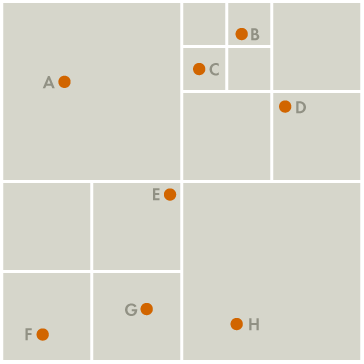
\includegraphics[width=0.30\textwidth]{assests/example-space}
  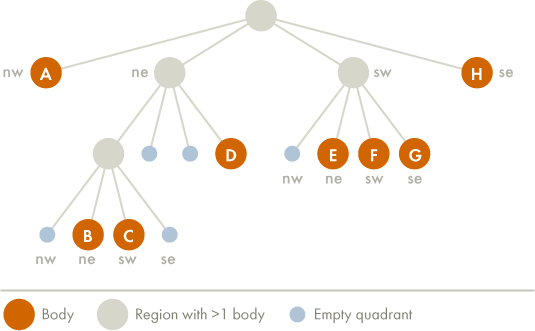
\includegraphics[width=0.65\textwidth]{assests/example-tree}
  \captionof{figure}{A 2D space subdivided into regions, with each region
    containing $0$ or $1$ body. The quadtree created from this 2D space can also
    be seen (nw referers to the north west quadrant etc.) \cite{BH-algo}.}
  \label{fig:subdivision}
\end{Figure}
We see that each region containing more than one body is colored gray in figure
\ref{fig:subdivision} (we call these nodes internal node), internal nodes will
then store a single body representation of it substree's bodies, so if we were
to calculate the interaction between node
$H$ and nodes $B,C,D$ and we find the distance to far, we would use the
representation stored in $D$'s parent. If they are not to far we travers the tree
recursively untill we reach the leaves. To determine wheather or not a node is to
far away we use the quotiens $\frac{s}{d}$ where $s$ is the width of a region and
$d$ is the distance between the center-of-mass, we hold this up against a threshold.
The threshold ($\theta$) ends up being the trade-off between accuracy and performance,
so if $\theta = 0$ no internal node is used as a representation, and we go back
to the performance of the naive implementation (actually a bit slower due to the
overhead of constructing the tree). A common value is $\theta = 0$.

The main advantage of using a quadtree (and by extension octree) is the even
divide in the regions, so if the space it $10$ units wide we know that the region
at level $3$ in the tree is $1.6667$, that is $s_r=\frac{w}{2l}$ where $s_r$ is the
width of region $r$, $w$ is the total width of the space, and $l$ is the level.
This means that $\theta$ is easy to calculate.

\subsubsection{Using a binary radix-tree}